\section{Results}
To demonstrate \deploy's capability to effectively conduct transition
scenario analysis and meet the objectives described in section 
\ref{sec:obj}, this section will 
(1) demonstrate \deploy's capability in simple transition scenarios, 
(2) compare the prediction methods for different transition scenarios, and
(3) demonstrate using \deploy to set up successful EG01-EG23, EG01-EG24, 
EG01-EG29, and EG01-EG30 transition scenarios. 
The input files and scripts to produce the results and plots in this
paper can be reproduced using \cite{dnoauthor_d3ploy:_2018}, and 
\cite{chee_arfc/transition-scenarios_2018}. 

\subsection{Demonstration of \deploy's capabilities}
\label{sec:demo}
Constant, linearly increasing, and sinusoidal power demand simulations 
are conducted to demonstrate \deploy's capabilities for 
simulating transition scenarios and to inform decisions about 
input parameters when setting up larger transition scenarios 
with many facilities.  
These simulations are basic transition scenarios that only include 
three types of facilities: \texttt{source}, \texttt{reactor}, and 
\texttt{sink}. 
All simulations have ten initial \texttt{reactor} facilities 
(\texttt{reactor1} to \texttt{reactor10}). 
These reactors have staggered cycle lengths and lifetimes to prevent 
simultaneous refueling and set up gradual decommissioning. 
\deploy is set up to deploy \texttt{new reactor} facilities
to meet the loss of power supply introduced from the decommissioning 
of the initial \texttt{reactor} facilities. 
The \deploy input parameters for each simulation is shown in Table 
\ref{tab:demonstrations}. 
Figure \ref{fig:powerplots} shows the user-defined power demand curves 
that \deploy needs to deploy facilities meet for each simulation.

\begin{table}[]
    \resizebox{\textwidth}{!}{%
    \begin{tabular}{|l|l|c|l|l|}
    \hline
    \multirow{2}{*}{}                         & \multicolumn{1}{c|}{\multirow{2}{*}{\textbf{Input Parameter}}} & \multicolumn{3}{c|}{\textbf{Simulation Description}}                                                                                                                                                                                                                                                       \\ \cline{3-5} 
                                              & \multicolumn{1}{c|}{}                                          & \multicolumn{1}{l|}{\textbf{Constant Power}}                                                                 & \textbf{\begin{tabular}[c]{@{}l@{}}Linearly Increasing \\ Power\end{tabular}}                  & \textbf{Sinusoidal Power}                                                                  \\ \hline
    \multirow{5}{*}{\textbf{Required}} & Demand driving commodity                                       & \multicolumn{3}{c|}{Power}                                                                                                                                                                                                                                                                                 \\ \cline{2-5} 
                                              & Demand equation                                                & \multicolumn{1}{l|}{10000 MW}                                                                                & \begin{tabular}[c]{@{}l@{}}t\textless 40: 10000 MW\\ t\textgreater{}=40: 250*t MW\end{tabular} & 1000*$\sin(\pi*t/3)$+10000                                                                 \\ \cline{2-5} 
                                              & Facilities it controls                                         & \multicolumn{3}{c|}{Source, reactor, sink}                                                                                                                                                                                                                                                                 \\ \cline{2-5} 
                                              & Prediction method                                              & \multicolumn{1}{l|}{\begin{tabular}[c]{@{}l@{}}Power: FFT\\ Fuel: MA\\ Spent fuel: MA\end{tabular}}          & \begin{tabular}[c]{@{}l@{}}Power: FFT\\ Fuel: MA\\ Spent fuel: FFT\end{tabular}                & \begin{tabular}[c]{@{}l@{}}Power: HW\\ Fuel: MA\\ Spent fuel: FFT\end{tabular}             \\ \cline{2-5} 
                                              & Deployment Driving Method                                      & \multicolumn{3}{c|}{Installed Capacity}                                                                                                                                                                                                                                                                    \\ \hline
    \multirow{2}{*}{\textbf{Optional}} & Buffer type                                                    & \multicolumn{3}{c|}{Absolute}                                                                                                                                                                                                                                                                              \\ \cline{2-5} 
                                              & Buffer size                                                    & \multicolumn{1}{l|}{\begin{tabular}[c]{@{}l@{}}Power: 3000 MW\\ Fuel: 0 kg \\ Spent fuel: 0 kg\end{tabular}} & \begin{tabular}[c]{@{}l@{}}Power: 2000 MW\\ Fuel: 1000 kg \\ Spent fuel: 0 kg\end{tabular}     & \begin{tabular}[c]{@{}l@{}}Power: 2000 MW\\ Fuel: 1000 kg \\ Spent fuel: 0 kg\end{tabular} \\ \hline
    \end{tabular}%
    }
    \caption{\deploy's input parameters for the basic transition scenarios.}
    \label{tab:demonstrations}
    \end{table}

    \begin{figure}[]
        \begin{center}
            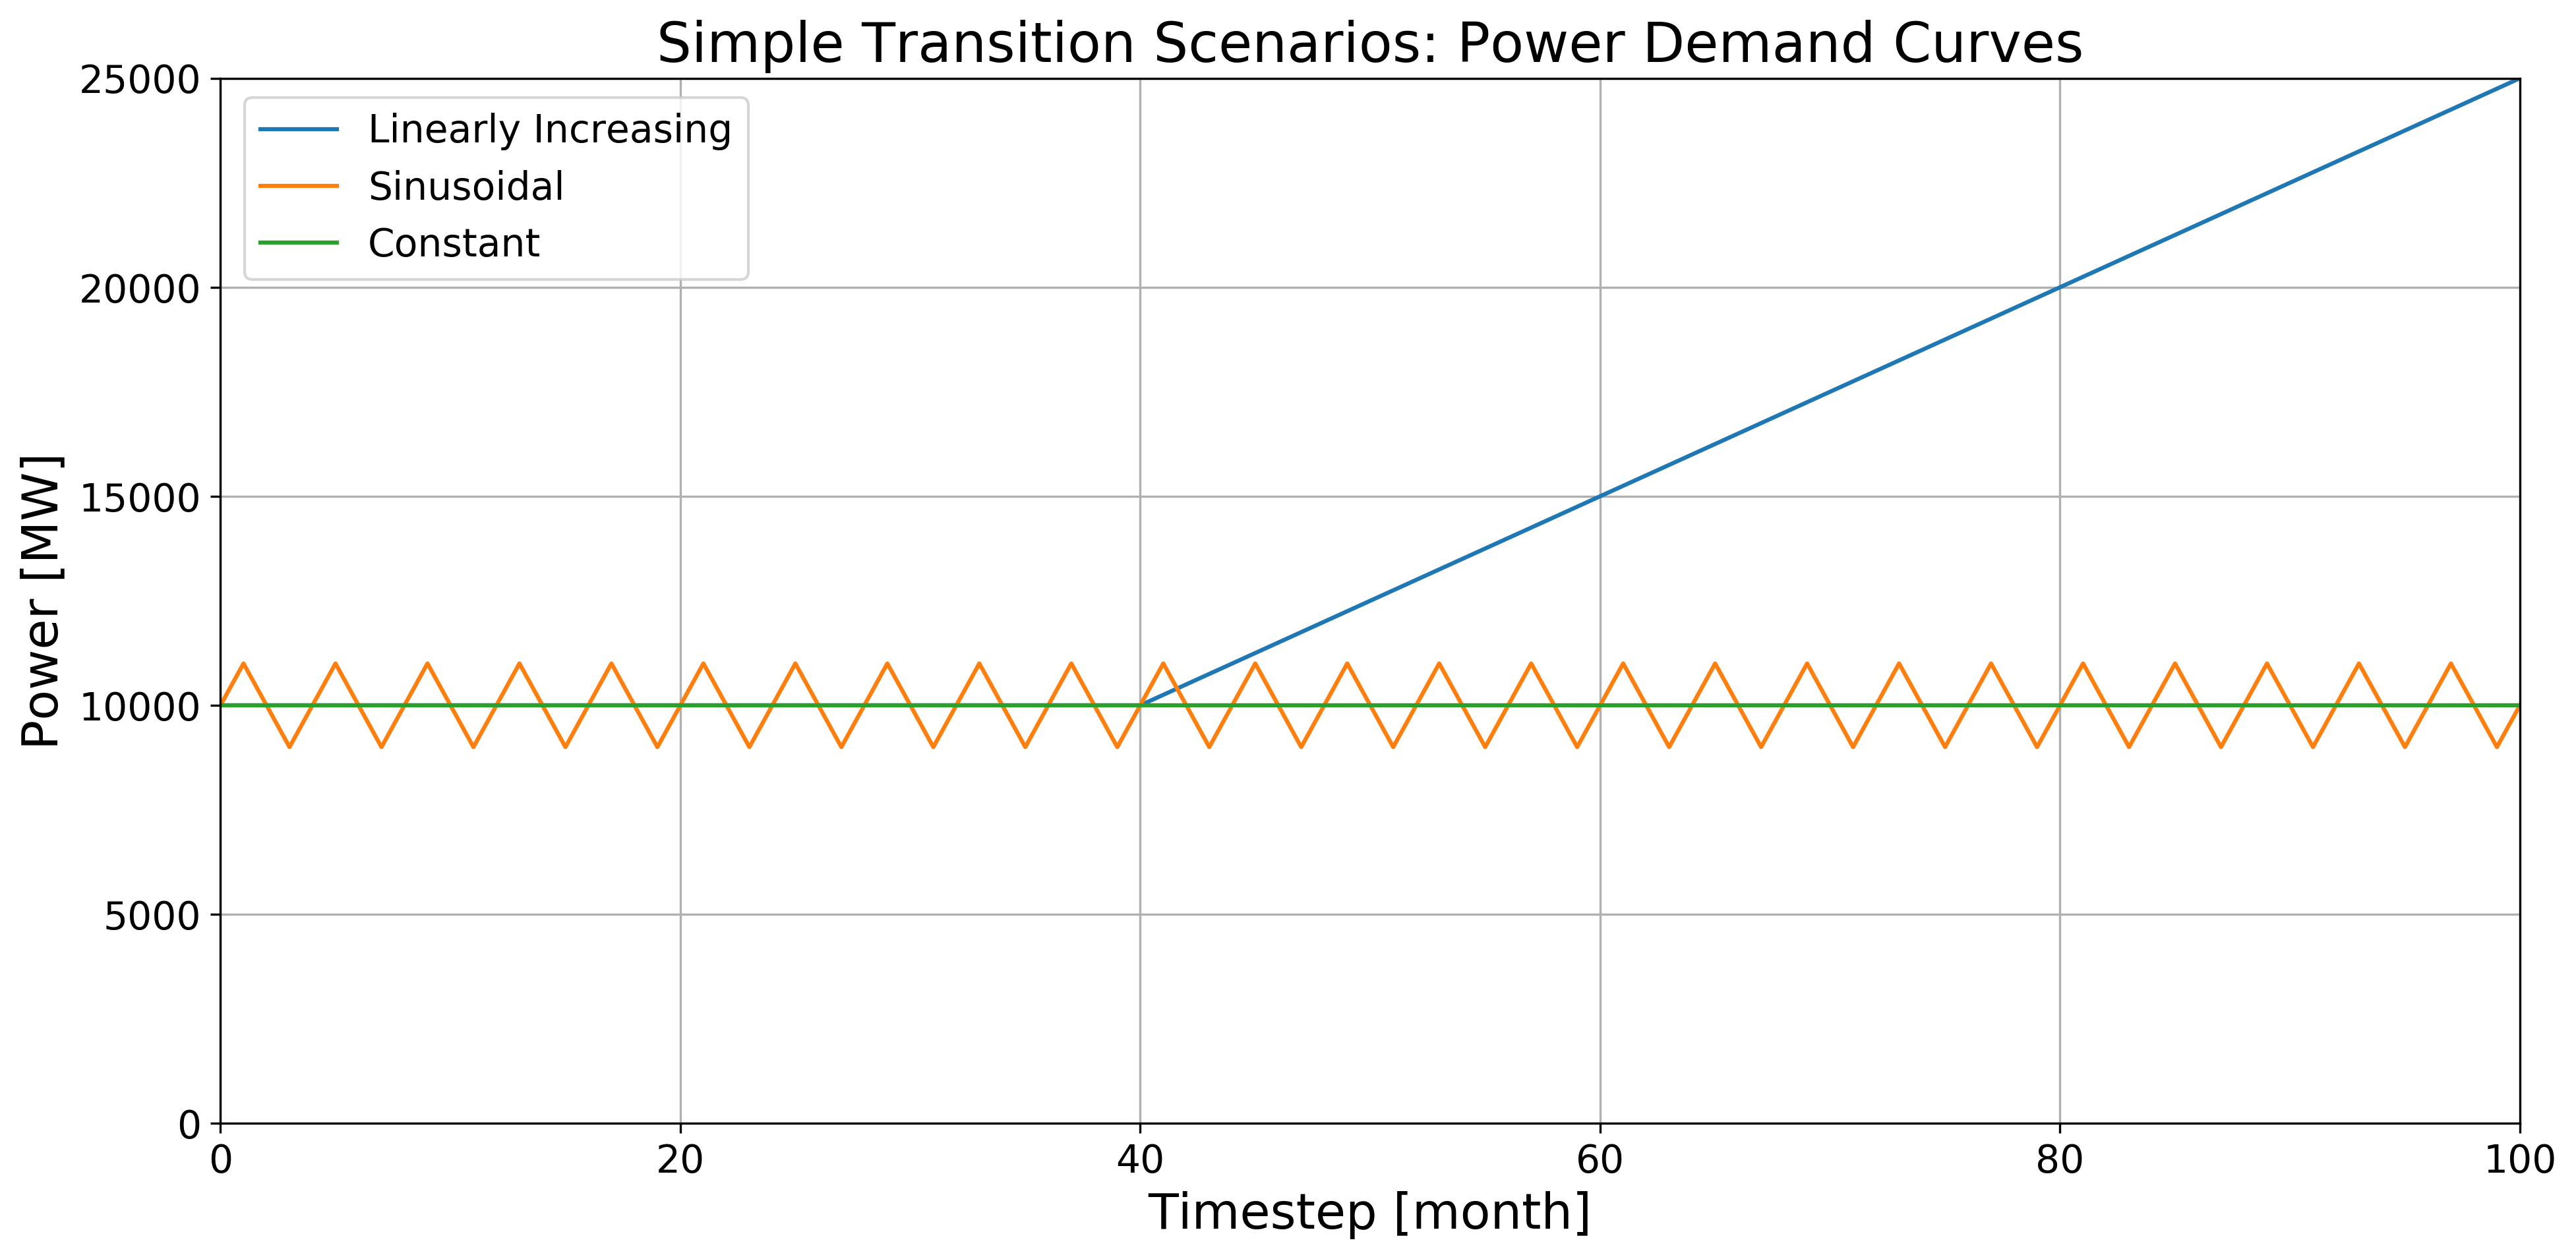
\includegraphics[scale=0.37]{./figures/powerplots.png}
        \end{center}
            \caption{Power demand curves for basic transition scenarios.}
        \label{fig:powerplots}
    \end{figure}

\subsubsection{Basic Transition Scenario Simulation: Constant Demand}
Figures \ref{fig:constanttransition-power}, \ref{fig:constanttransition-fuel}
and \ref{fig:constanttransition-spentfuel} demonstrate \deploy's capability 
to deploy reactor and supporting facilities to meet the user 
determined constant power demand and subsequently demanded 
secondary commodities with minimal undersupply. 
Table \ref{tab:transition-scenario-results} shows the number of 
undersupplied timesteps. 
Figure \ref{fig:constanttransition-power} demonstrates that
the main objective of \deploy was met since there are no timesteps
in which the supply of power falls under demand.
By using a combination of the fast fourier transform method for 
predicting demand and setting the supply buffer to 3000MW 
(the capacity of 3 reactors), the user minimizes the number of 
undersupplied timesteps for every commodity.

In figure \ref{fig:constanttransition-fuel},
a facility with a large fuel throughput is initially
deployed to meet the large initial fuel demand for the starting
up of ten reactors. 
\deploy is prevented from deploying many supporting
facilities that end up being redundant at the later parts of 
the simulation, by having an initial facility with a large throughput
exist for the first few timesteps in the simulation.
This is a reflection of reality in which reactor manufacturers will 
accumulate an appropriate amount of fuel inventory before starting 
up reactors. 
There is one timestep where there is an undersupply after the 
decommissioning of the large initial facility.  
This is unavoidable since the prediction methods in \deploy are 
unable to predict this sudden drop in demand. 

    \begin{figure}[]
        \centering
        \begin{subfigure}[t]{\textwidth}
        \centering
            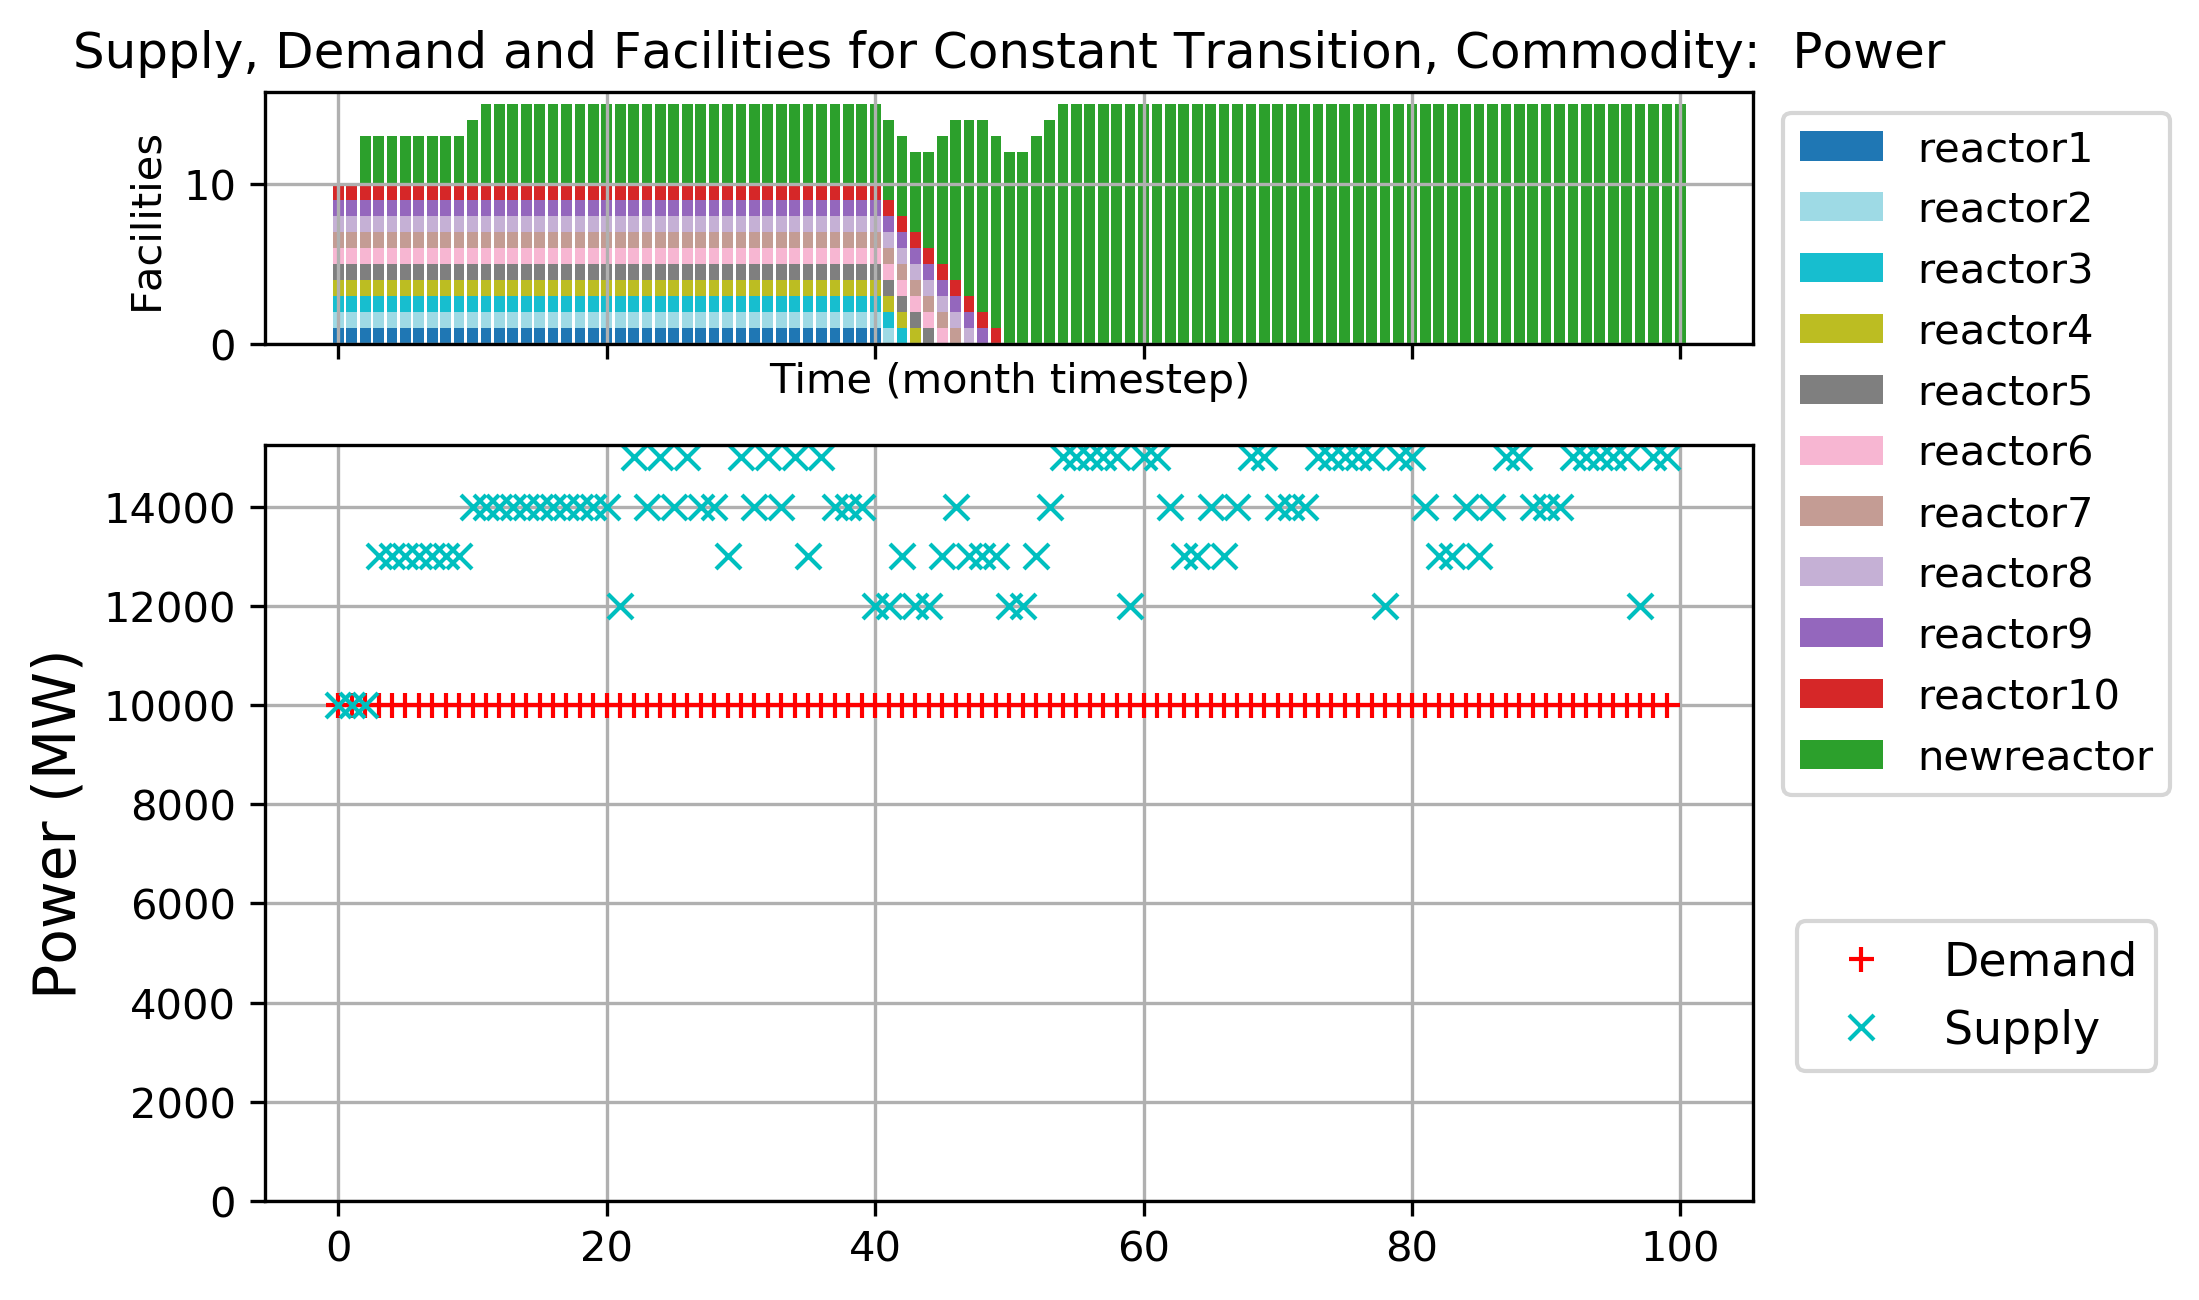
\includegraphics[width=0.8\linewidth]{figures/constanttransition-power.png} 
            \caption{The power demand is a user-defined equation and power is supplied by the reactors.}
            \label{fig:constanttransition-power}
        \end{subfigure}
        \begin{subfigure}[t]{0.65\textwidth}
            \centering
            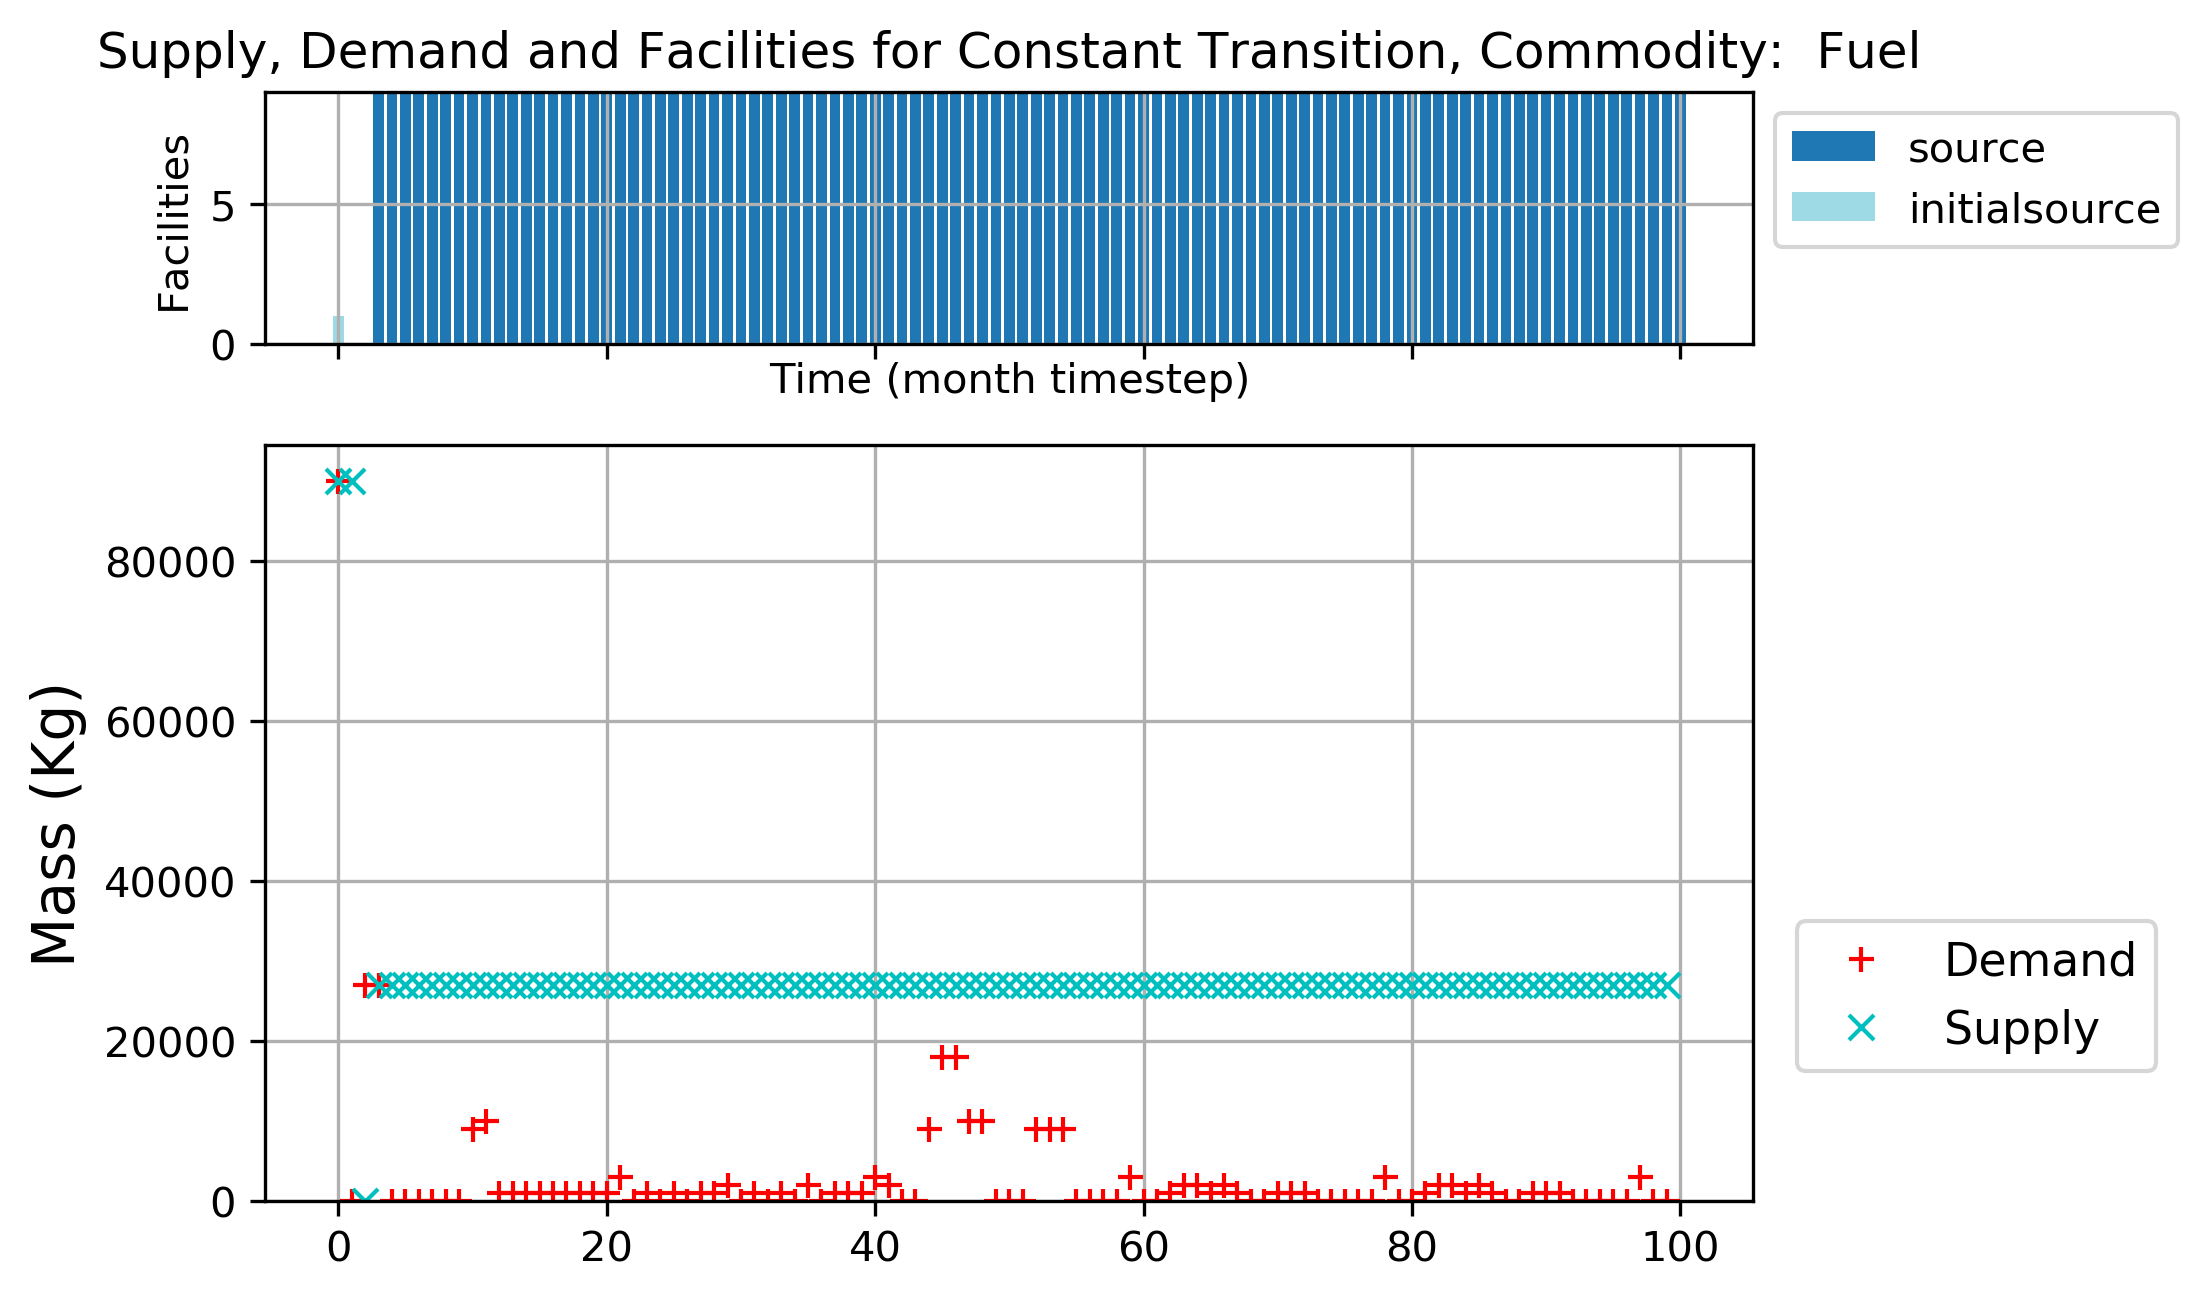
\includegraphics[width=\linewidth]{figures/constanttransition-fuel.png} 
            \caption{Fuel is demanded by reactors and supplied by source facilities.}
            \label{fig:constanttransition-fuel}
        \end{subfigure}
        \begin{subfigure}[t]{0.65\textwidth}
            \centering
            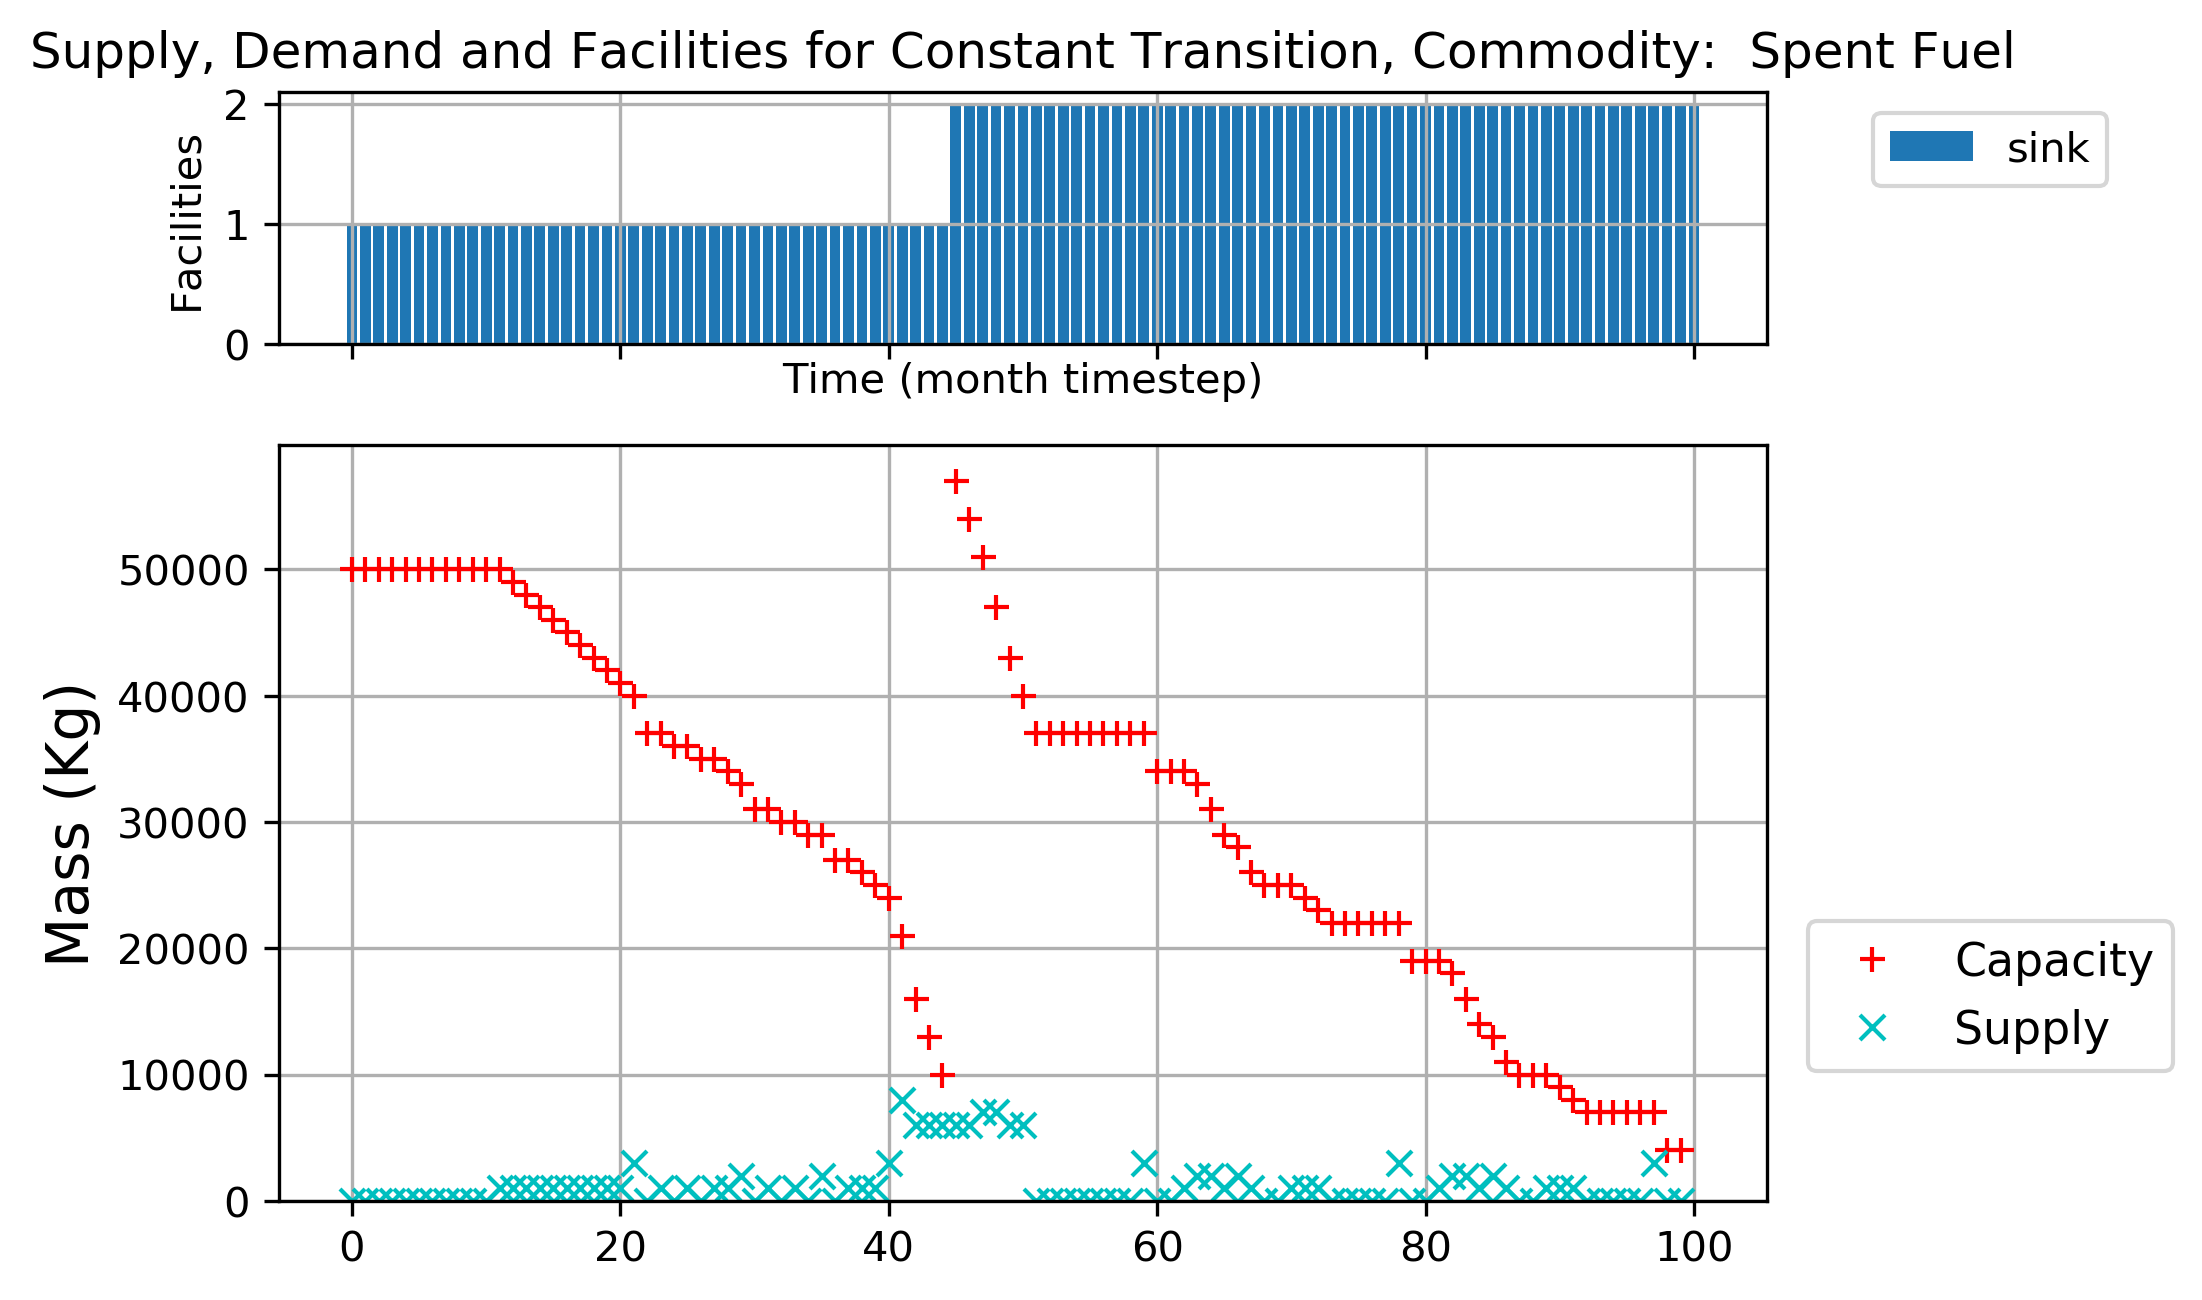
\includegraphics[width=\linewidth]{figures/constanttransition-spentfuel.png} 
            \caption{Spent Fuel is supplied by reactors and the capacity is provided by sink facilities.}
            \label{fig:constanttransition-spentfuel}
        \end{subfigure}
        \caption{Transition Scenario: Constant Power Demand of 10000MW}
    \end{figure}

\subsubsection{Basic Transition Scenario Simulation: Linearly Increasing Demand}

Figures \ref{fig:growingtransition-power}, \ref{fig:growingtransition-fuel}
and \ref{fig:growingtransition-spentfuel} demonstrate the capability 
of \deploy to deploy reactor and supporting facilities to meet the
power demand and subsequently demanded secondary commodities 
for a linearly increasing power demand. 
A smaller supply buffer could be used while still minimizing under supply.
Table \ref{tab:transition-scenario-results} shows the number of 
undersupplied timesteps. 
Figure \ref{fig:growingtransition-power} demonstrates that
the main objective of \deploy was met since there are no timesteps
in which the supply of power falls under demand.

\begin{figure}[]
    \centering
    \begin{subfigure}[t]{\textwidth}
    \centering
        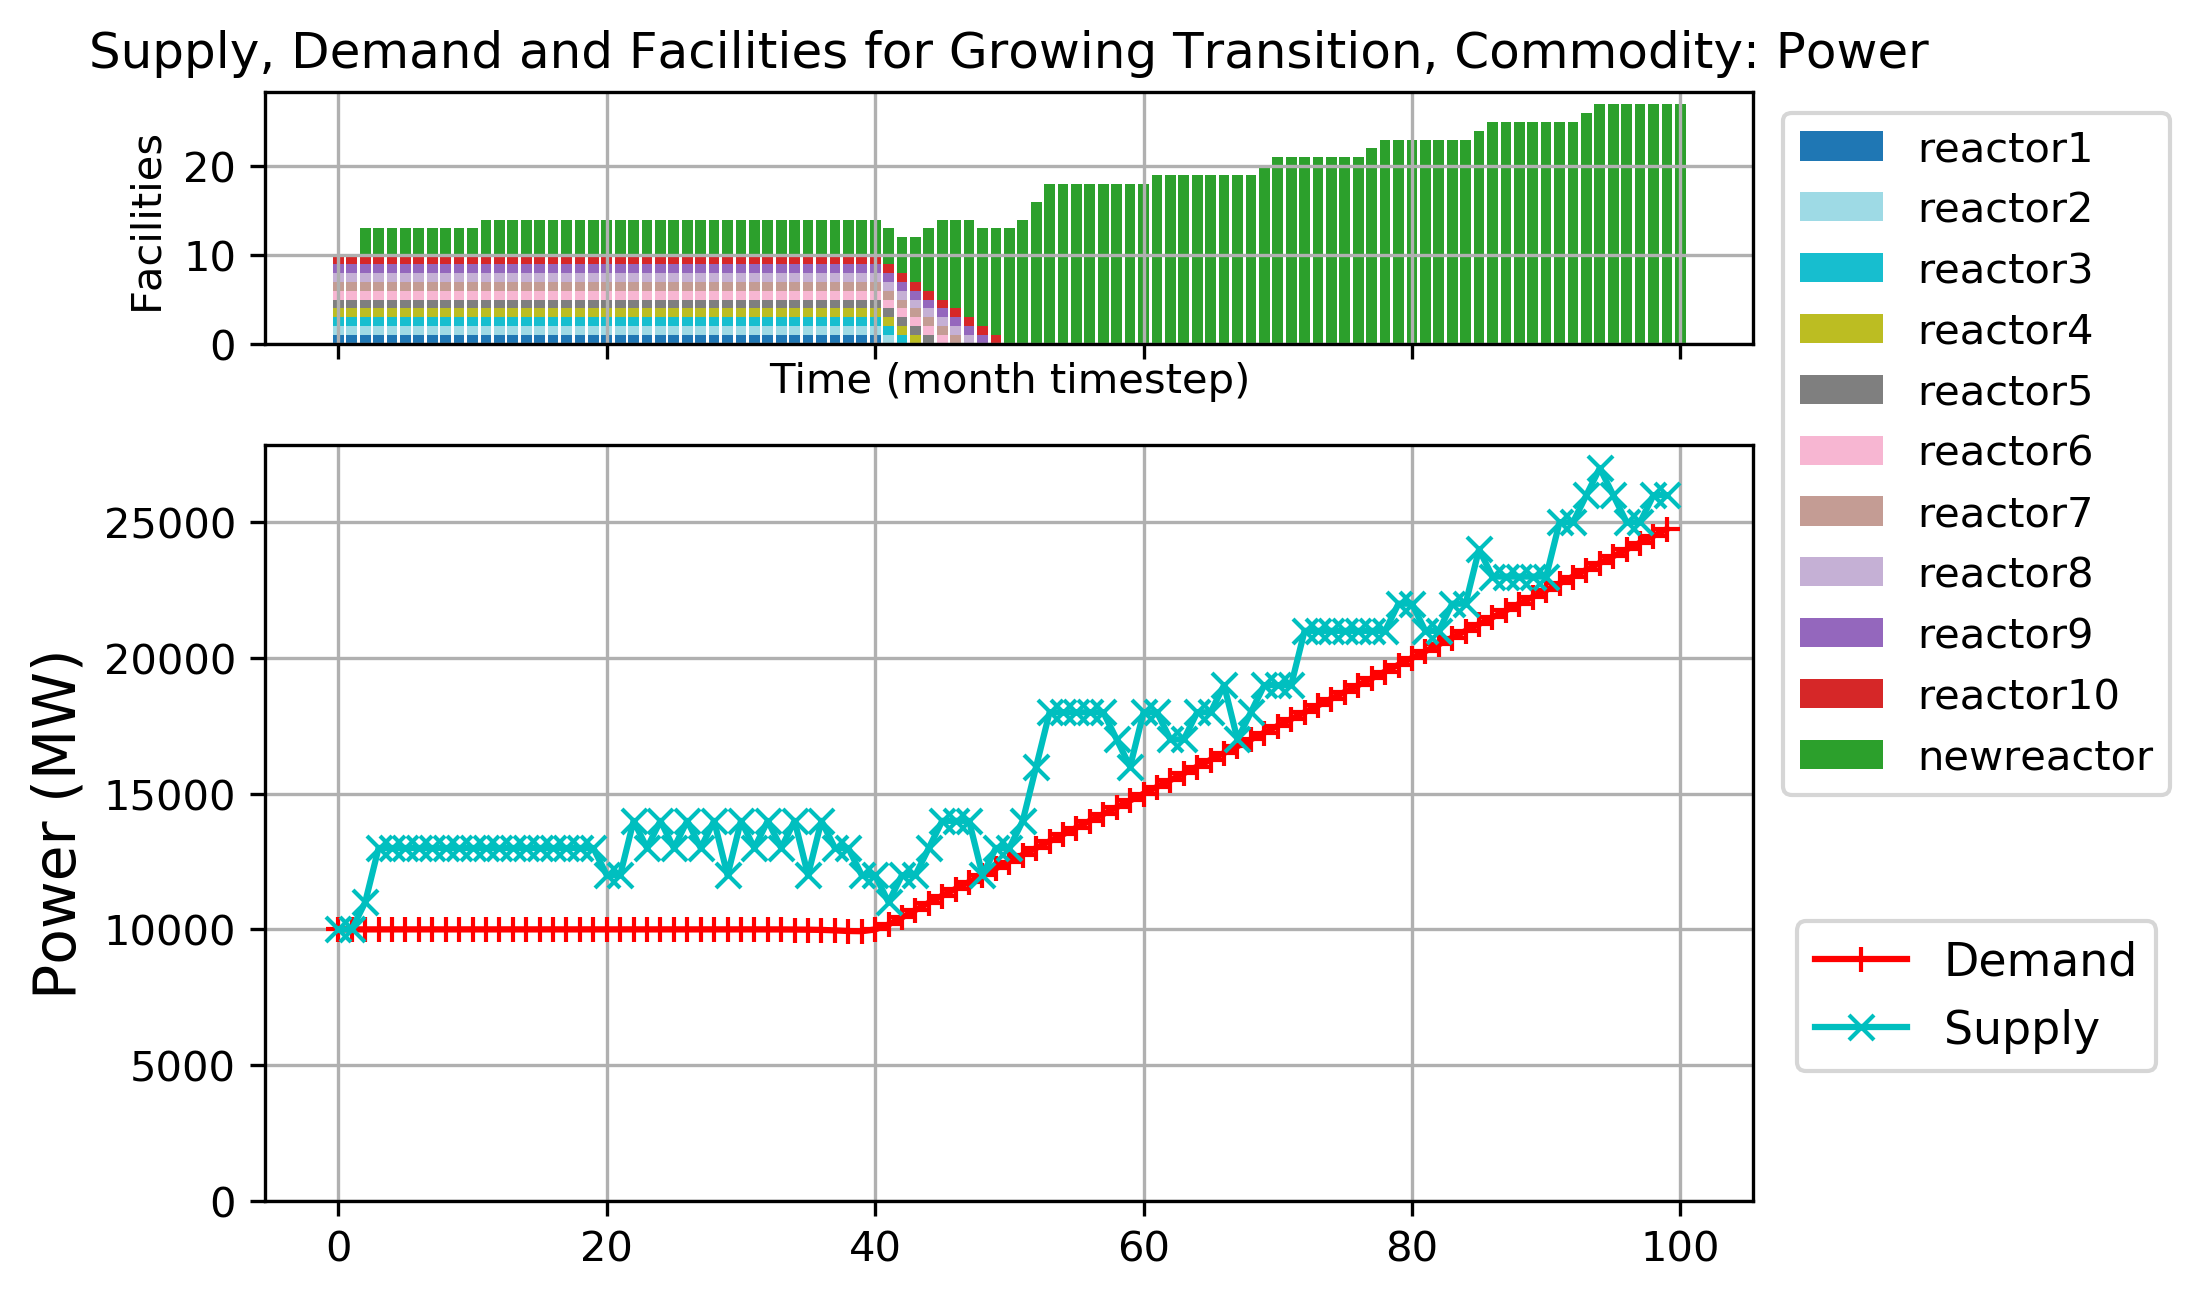
\includegraphics[width=0.8\linewidth]{figures/growingtransition-power.png} 
        \caption{The power demand is a user-defined equation and power is supplied by the reactors.}
        \label{fig:growingtransition-power}
    \end{subfigure}
    \begin{subfigure}[t]{0.65\textwidth}
        \centering
        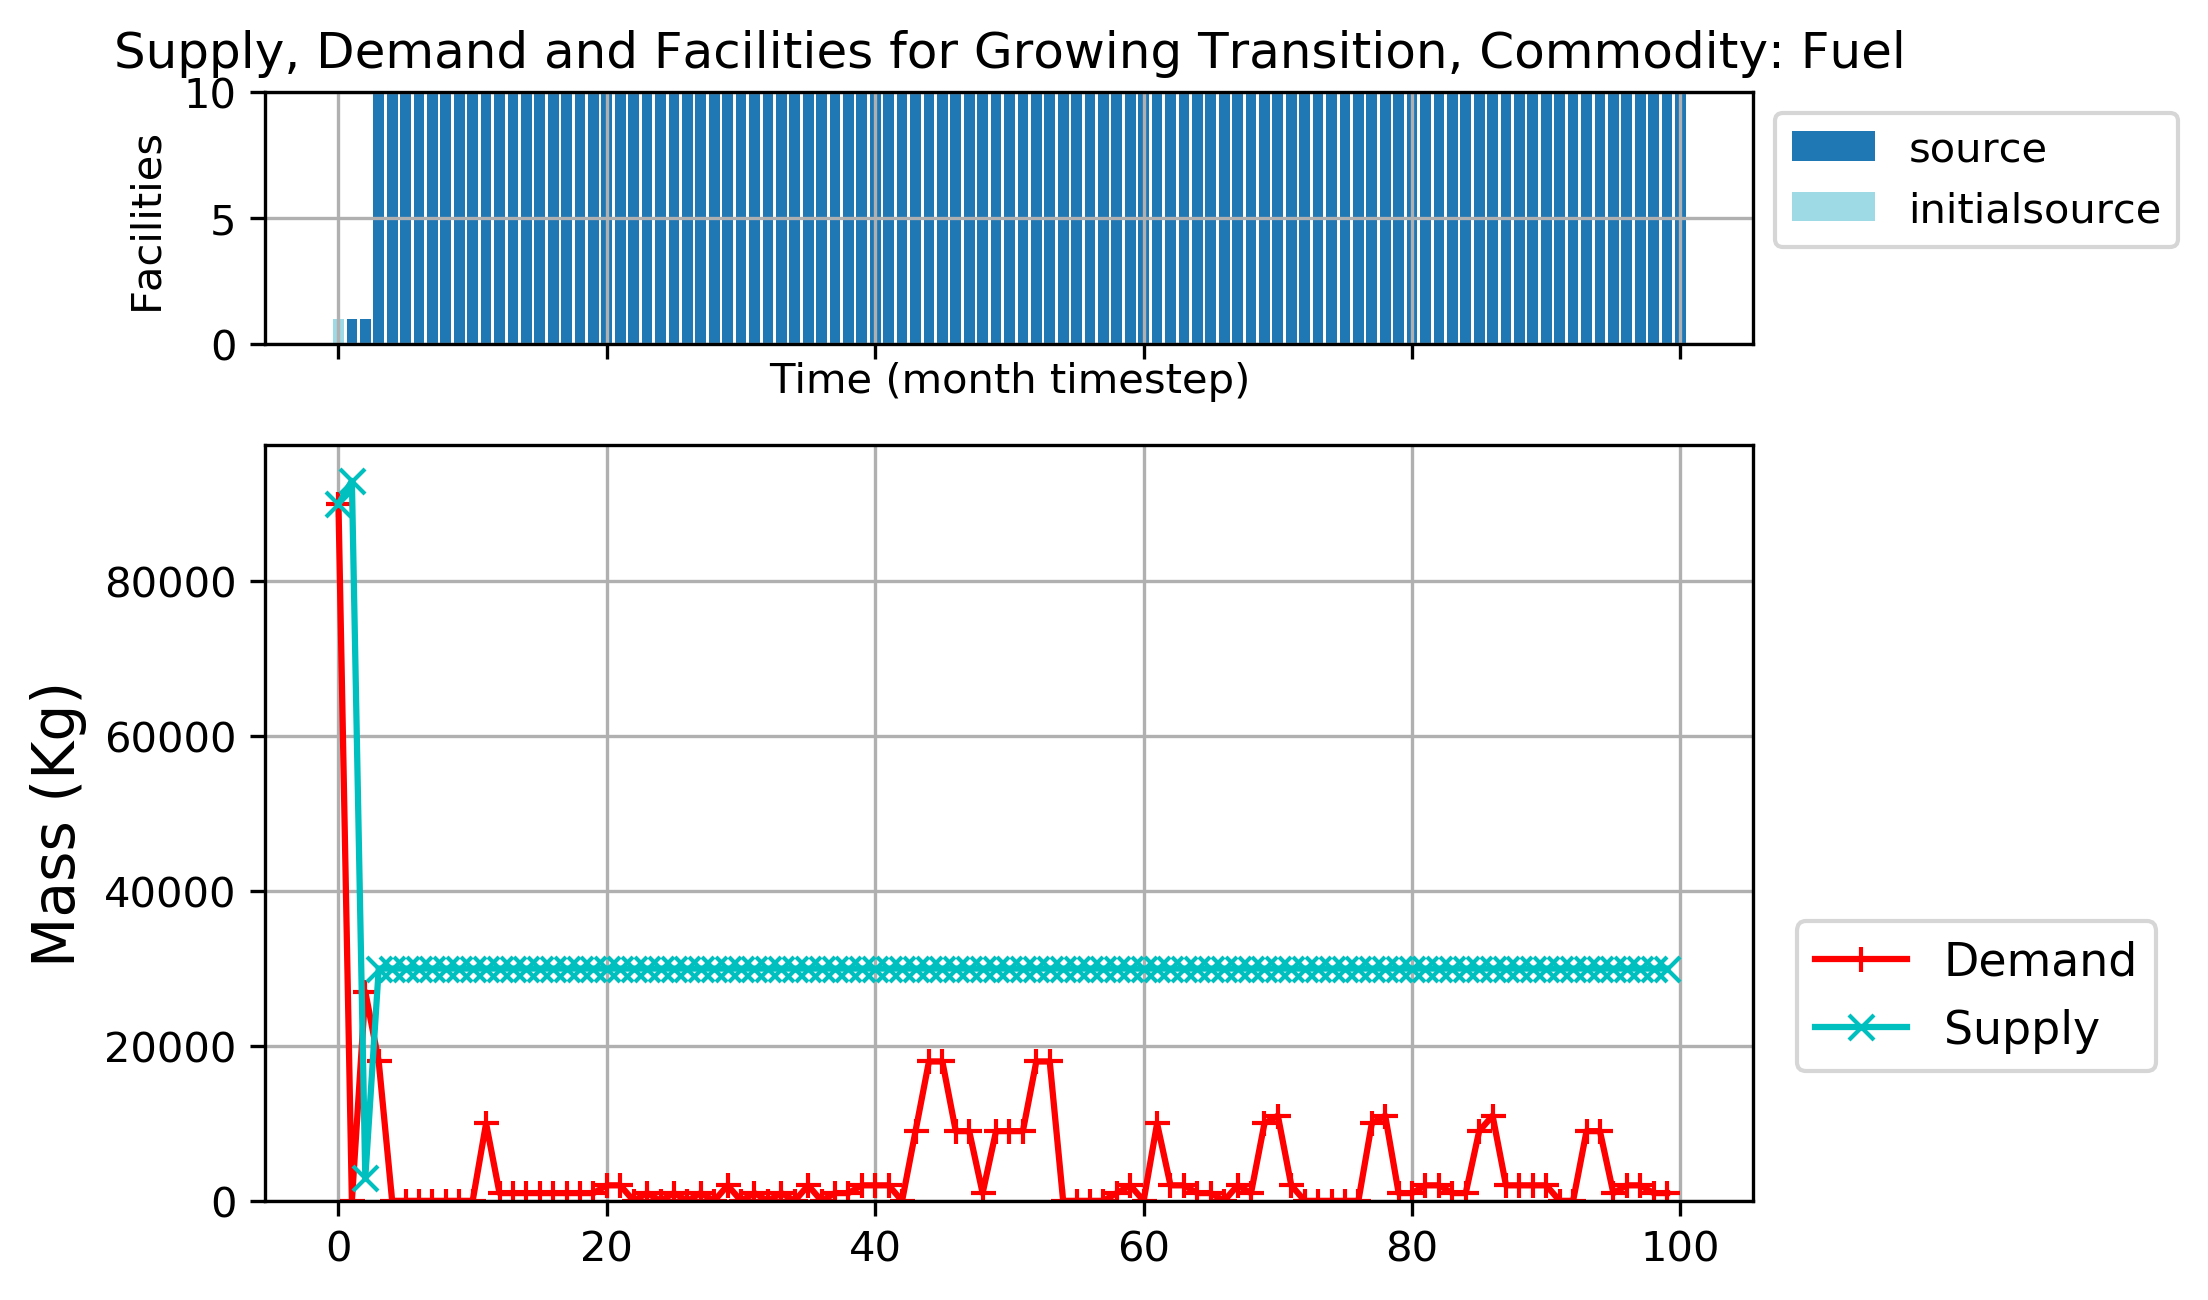
\includegraphics[width=\linewidth]{figures/growingtransition-fuel.png} 
        \caption{Fuel is demanded by reactors and supplied by source facilities.}
	    \label{fig:growingtransition-fuel}
    \end{subfigure}
    \begin{subfigure}[t]{0.65\textwidth}
        \centering
        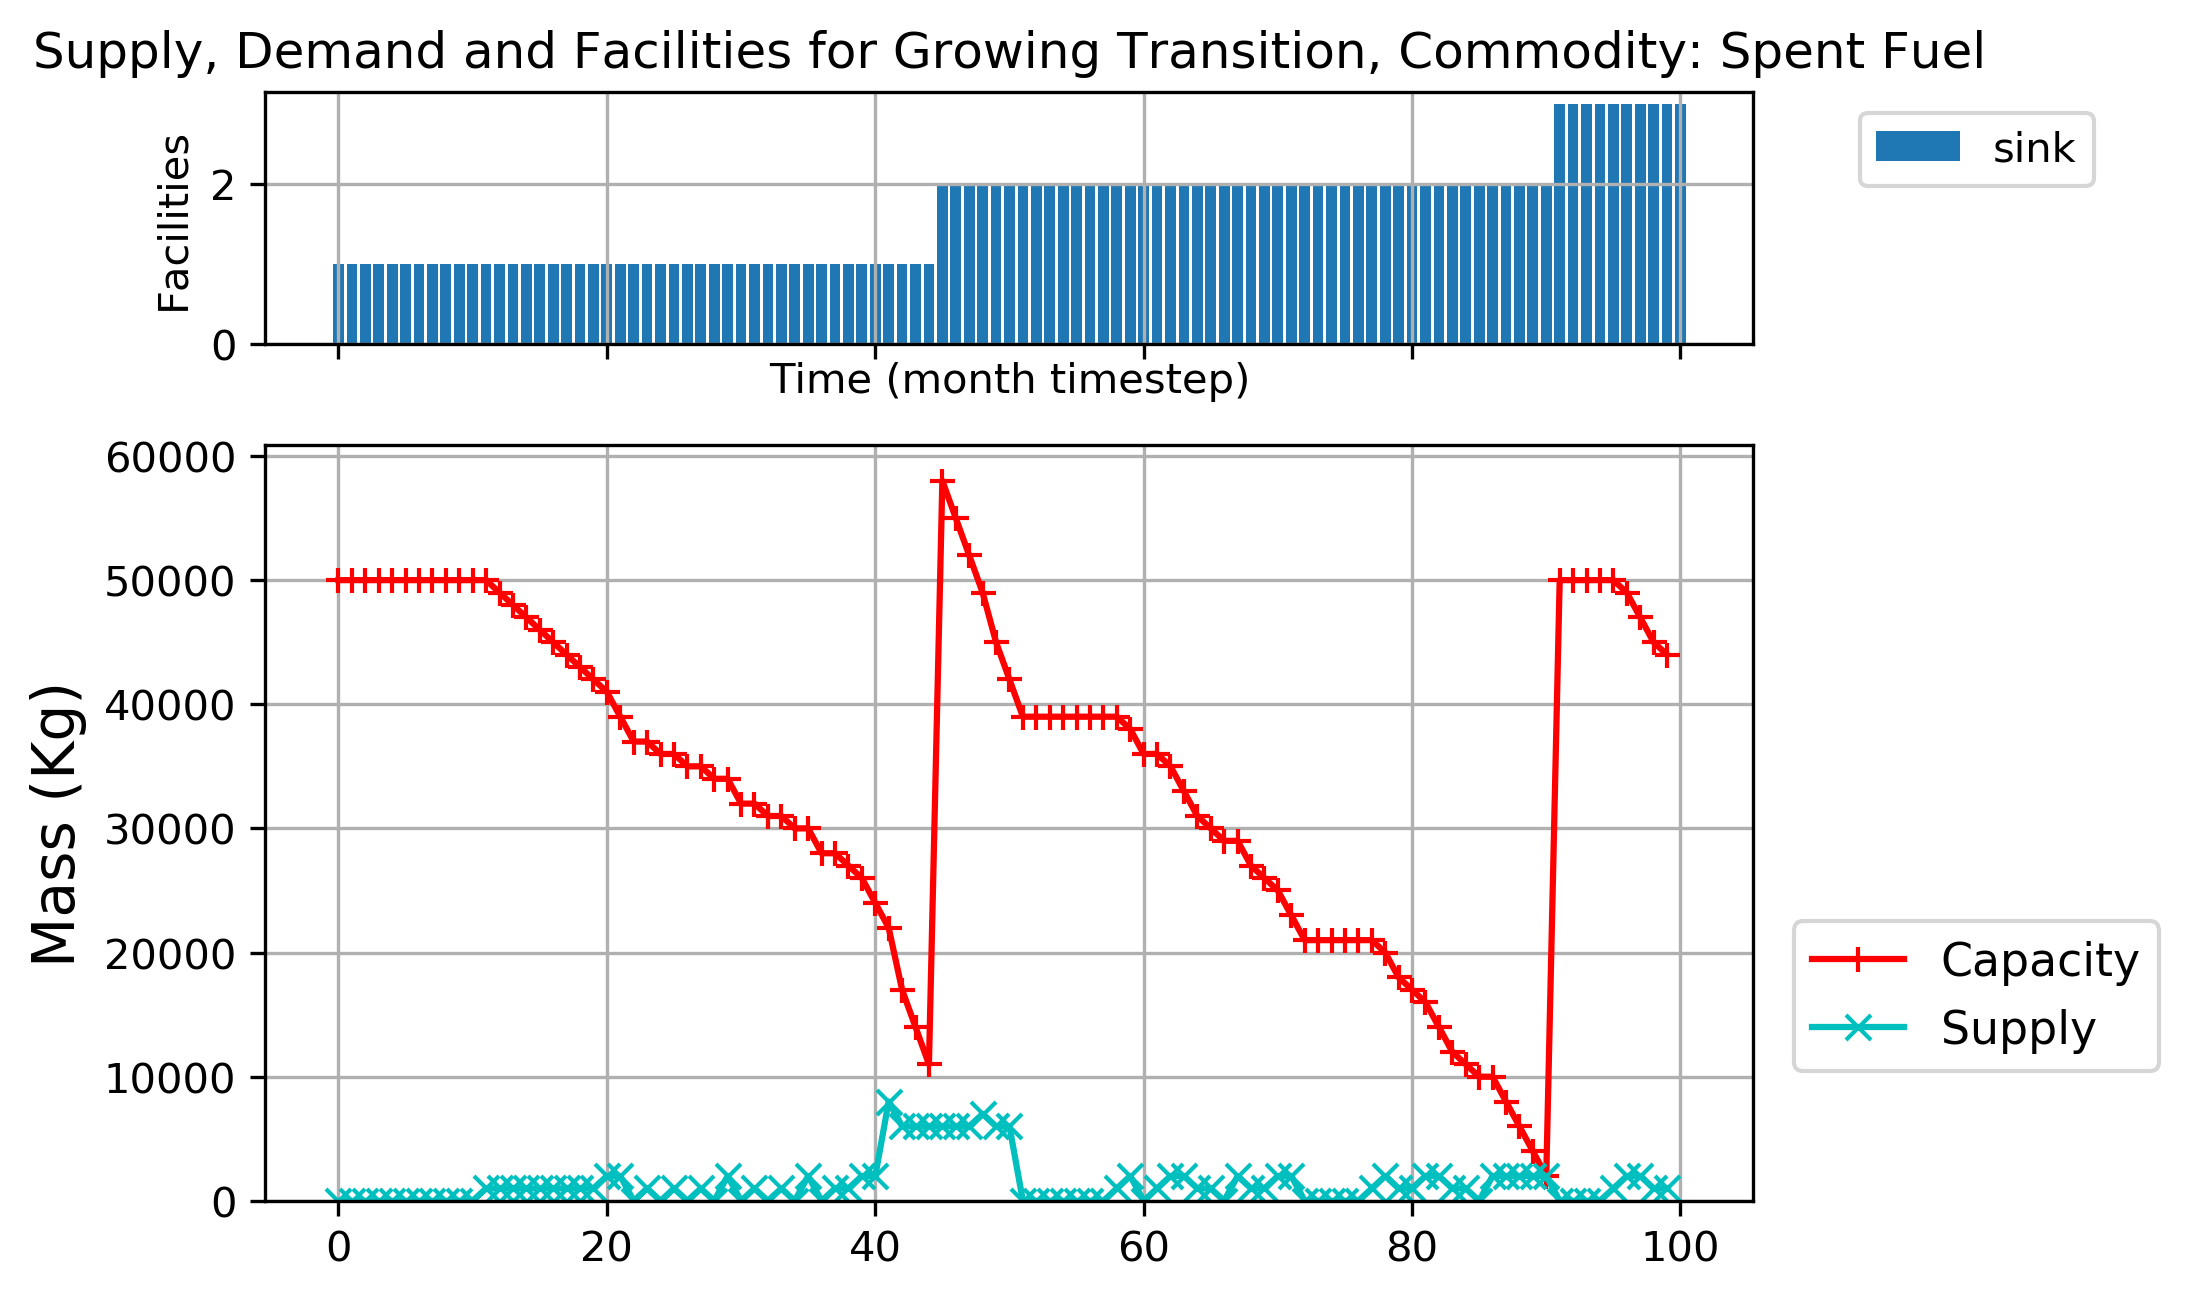
\includegraphics[width=\linewidth]{figures/growingtransition-spentfuel.png} 
        \caption{Spent Fuel is supplied by reactors and the capacity is provided by sink facilities.}
        \label{fig:growingtransition-spentfuel}
    \end{subfigure}
    \caption{Transition Scenario: Linearly increasing power demand.}
\end{figure}

\subsubsection{Basic Transition Scenario Simulation: Sinusoidal Demand}
A sinusoidal power demand is the reflection of power demand in 
the real world where power usage is higher in the winter and summer
and lower in the spring and fall. 
Figures \ref{fig:sinetransition-power}, \ref{fig:sinetransition-fuel}
and \ref{fig:sinetransition-spentfuel} demonstrate the capability 
of \deploy to deploy reactor and supporting facilities to meet the
power demand and subsequently demanded secondary commodities 
for a sinusoidal power demand. 
Table \ref{tab:transition-scenario-results} shows the number of 
undersupplied timesteps.

For a sinusoidal power demand, the use of the triple exponential method
for predicting demand is more effective than the 
fast fourier transform method which was used for the constant 
and linearly increasing power demand transition scenarios. 
This is because the triple exponential smoothing method excels in
forecasting data points for repetitive seasonal series of data. 

\begin{figure}[]
    \centering
    \begin{subfigure}[t]{\textwidth}
    \centering
        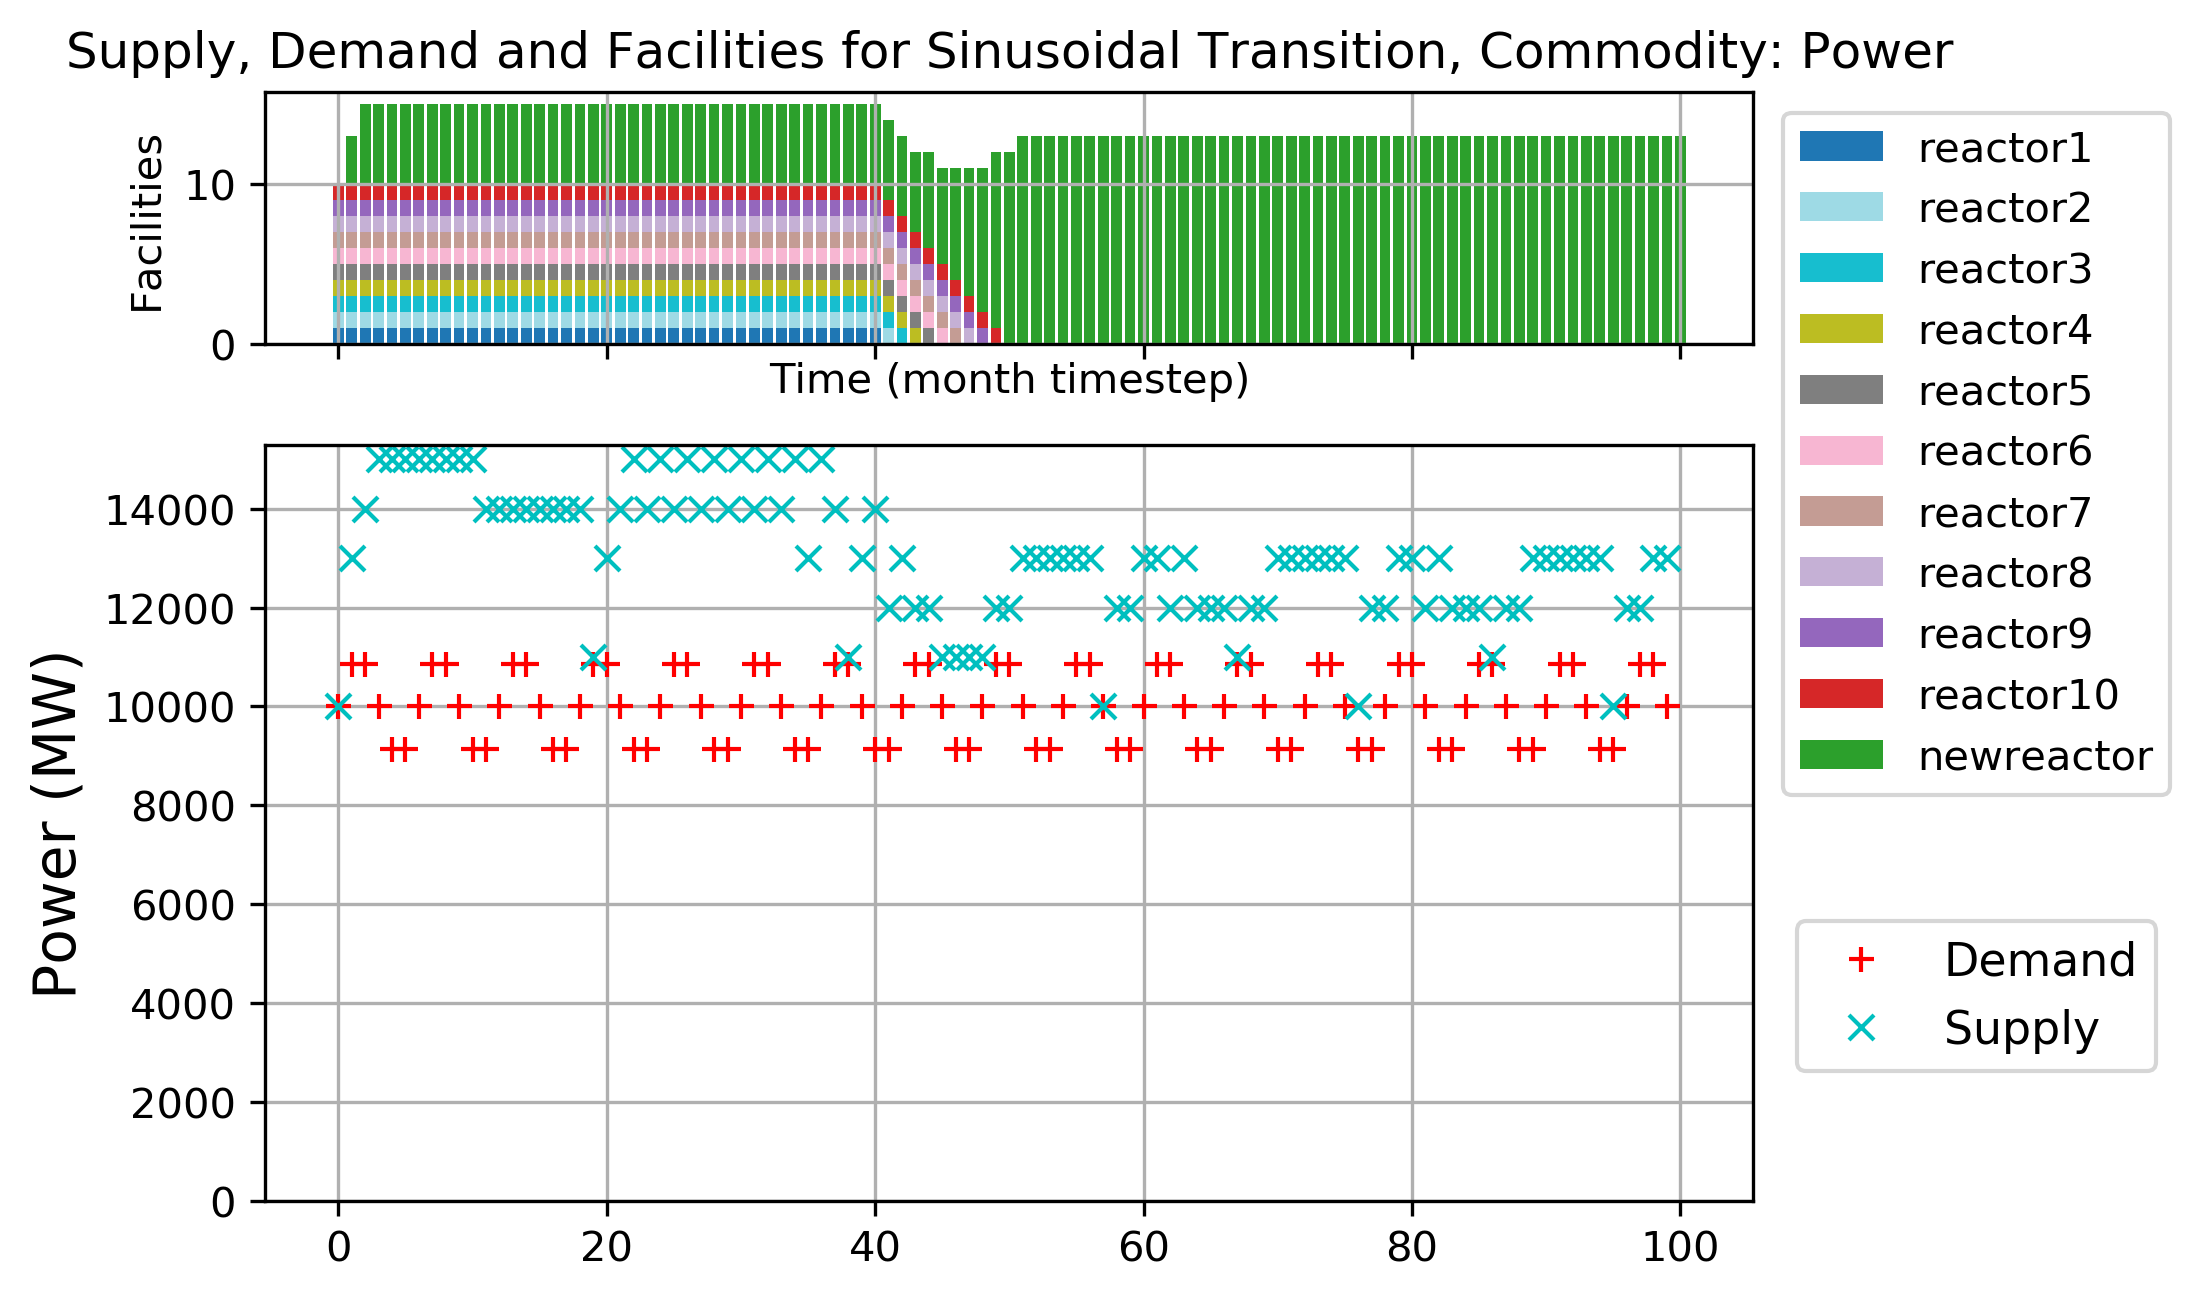
\includegraphics[width=0.8\linewidth]{figures/sinetransition-power.png} 
        \caption{The power demand is a user-defined equation and power is supplied by the reactors.}
        \label{fig:sinetransition-power}
    \end{subfigure}
    \begin{subfigure}[t]{0.65\textwidth}
        \centering
        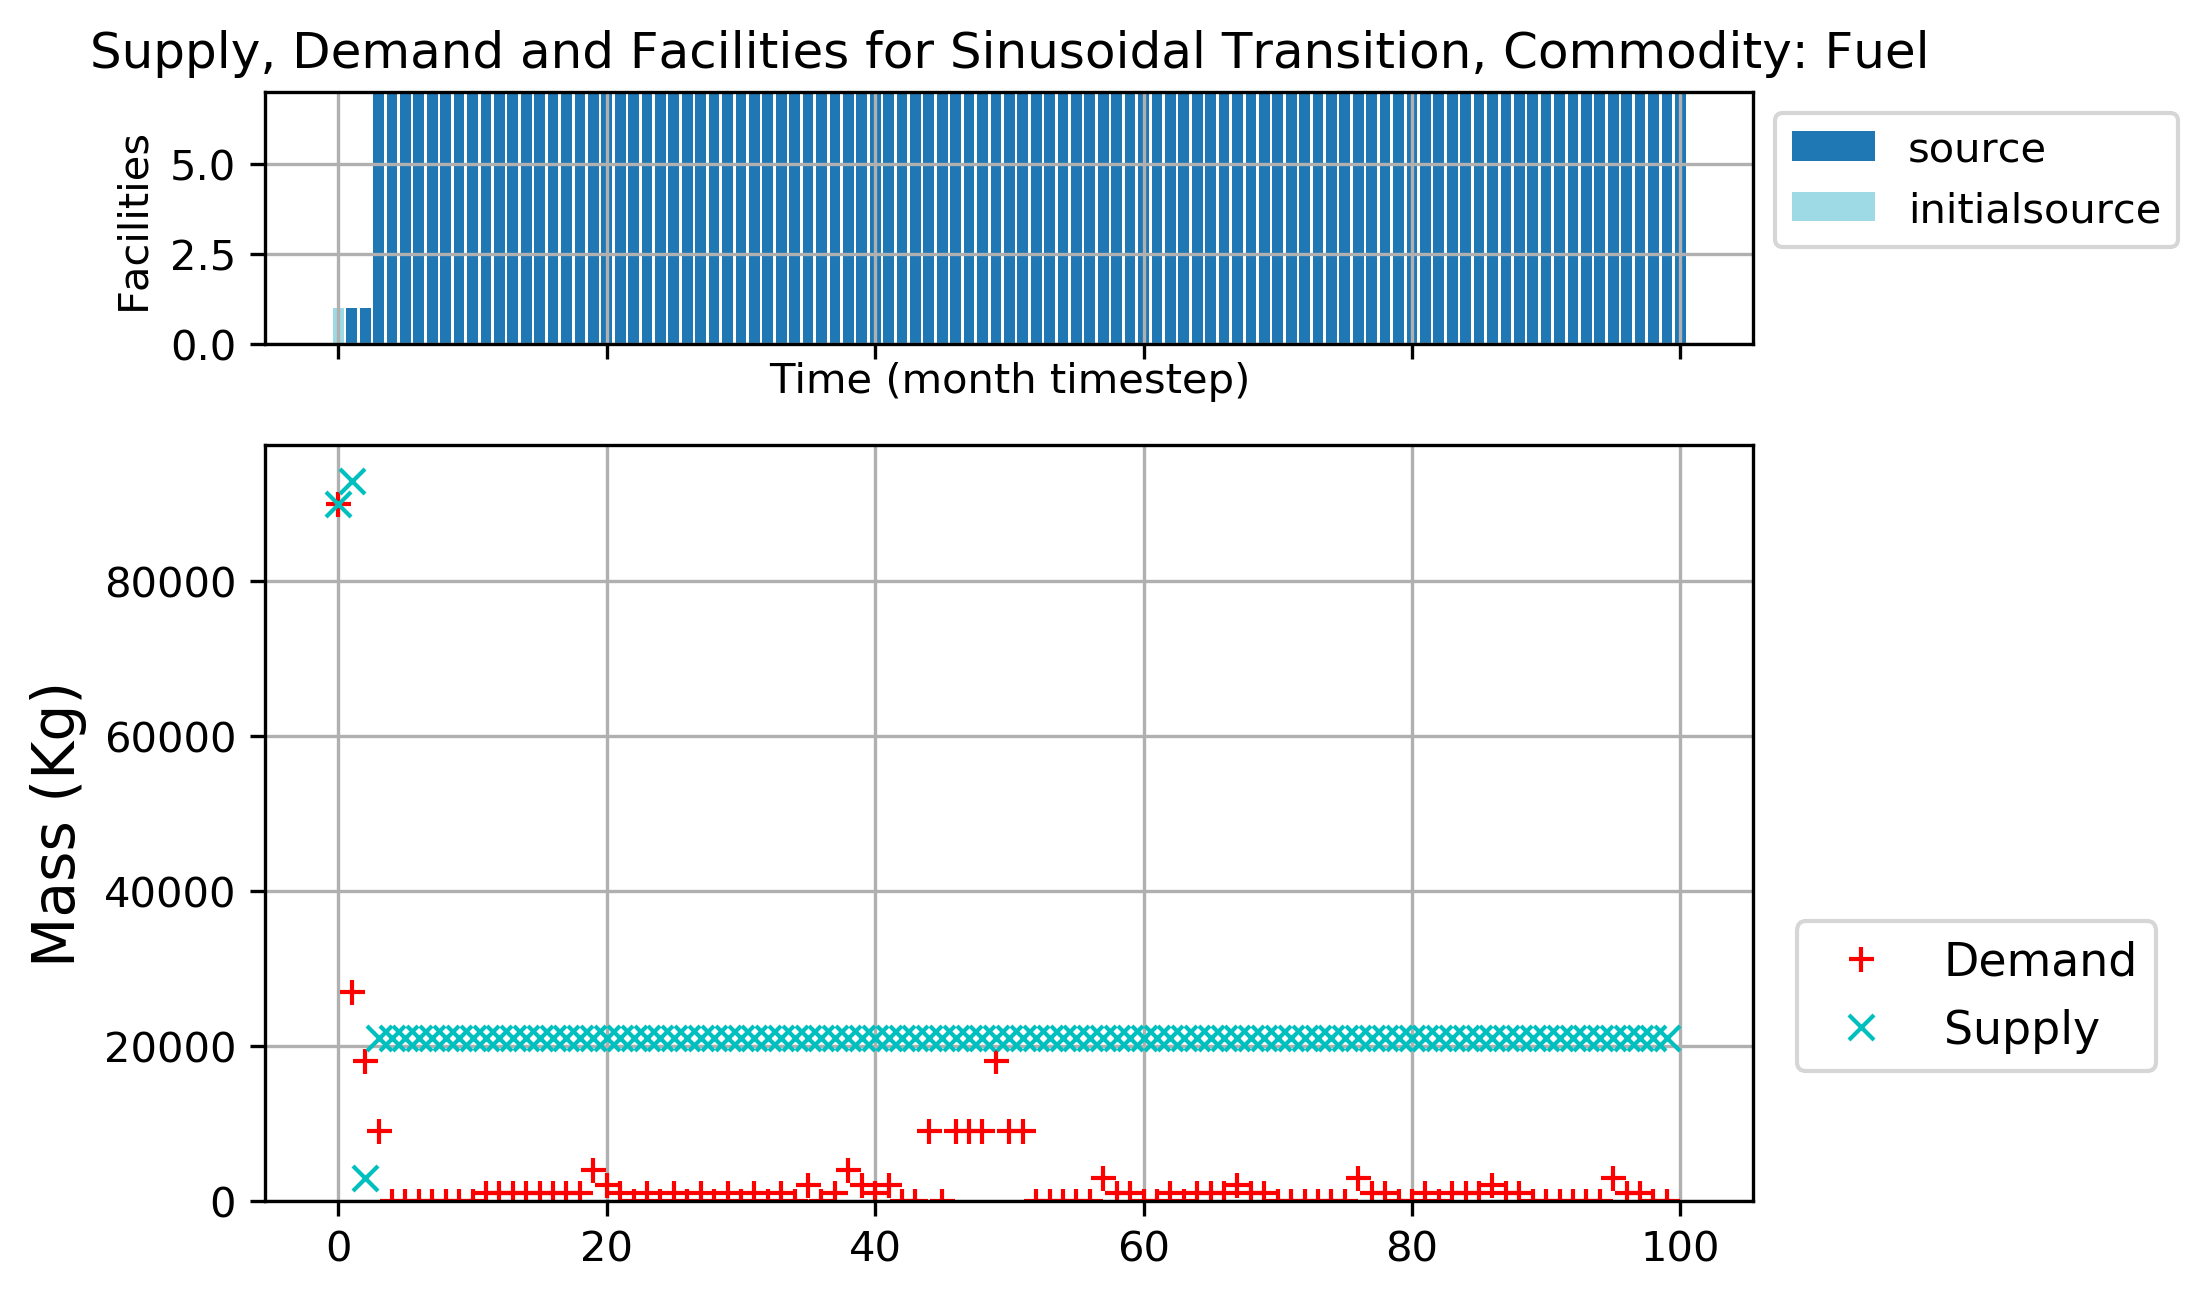
\includegraphics[width=\linewidth]{figures/sinetransition-fuel.png} 
        \caption{Fuel is demanded by reactors and supplied by source facilities.}
	    \label{fig:sinetransition-fuel}
    \end{subfigure}
    \begin{subfigure}[t]{0.65\textwidth}
        \centering
        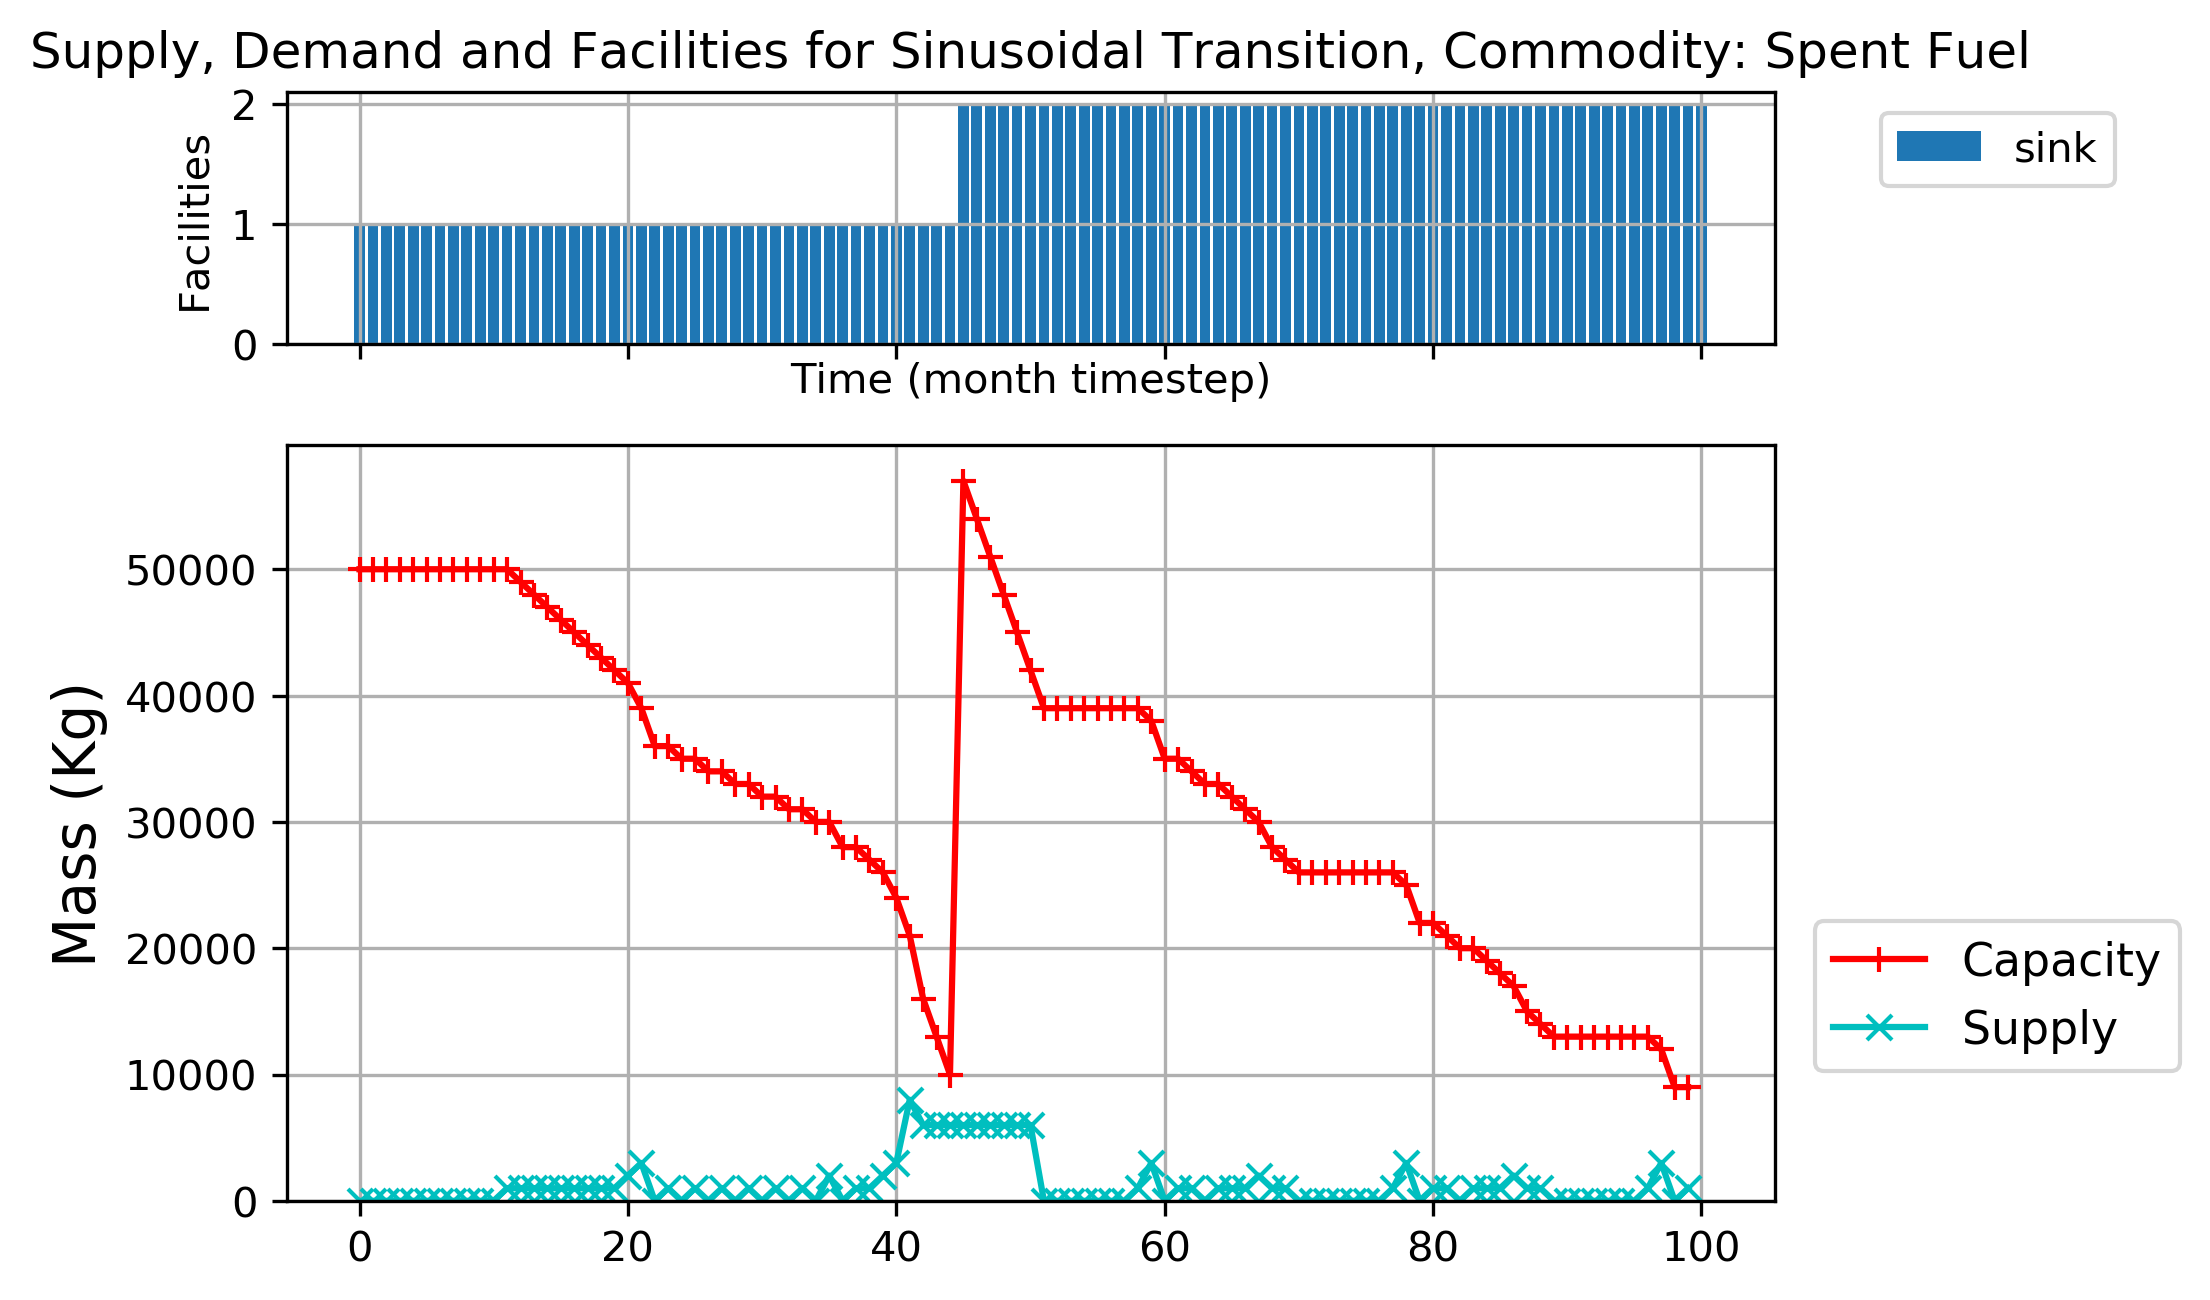
\includegraphics[width=\linewidth]{figures/sinetransition-spentfuel.png} 
        \caption{Spent Fuel is supplied by reactors and the capacity is provided by sink facilities.}
        \label{fig:sinetransition-spentfuel}
    \end{subfigure}
    \caption{Transition Scenario: Sinusoidal Power Demand}
\end{figure}

\begin{table}[]
    \centering
    \caption {Undersupply results for each commodity in each scenario}
    \label{tab:transition-scenario-results}
    \scalebox{0.7}{
    \begin{tabular}{|l|l|p{4cm}|}
    \hline
    \textbf{Basic Transition Scenario}    & \textbf{Commodity}    & \textbf{No. of timesteps with undersupply} \\ \hline
    \multirow{2}{*}{\textbf{Constant Power}} & Fuel & 1 \\ \cline{2-3}
                                             & Power & 0 \\ \cline{2-3}
                                             & Spent Fuel & 0 \\ \hline
    \multirow{2}{*}{\textbf{Linearly Increasing Power}} & Fuel & 1 \\ \cline{2-3}
                                             & Power & 0 \\ \cline{2-3}
                                             & Spent Fuel & 0 \\ \hline
    \multirow{2}{*}{\textbf{Sinusoidal Power}} & Fuel & 1 \\ \cline{2-3}
                                             & Power & 1 \\ \cline{2-3}
                                             & Spent Fuel & 0 \\ \hline
    \end{tabular}
    }
\end{table}